\subsection{Idealized biogeochemical model : NChlPZD, N$2$ChlPZD$2$, N$2$P$2$Z$2$D$2$}
ROMSTOOLS can help for the design of ROMS biogeochemical
experiments. For the initial conditions and lateral boundary
conditions, WOA provides a seasonal climatology for nitrateD
concentration and WOA or SeaWifs can be used to obtain a 
seasonal climatology of surface chlorophyll concentration.
Phytoplankton is estimated by a constant chlorophyll/phytoplankton 
ratio derived from previous simulations. Zooplankton is estimated
in a similar way. The part which should be edited by the user in 
romstools\_param.m is:\\
\\ 
\%\%\%\%\%\%\%\%\%\%\%\%\%\%\%\%\%\%\%\%\%\%\%\%\%\%\%\%\%\%\%\\
\%\\
\% Open boundaries and initial conditions parameters\\
\%   used by make\_clim.m, make\_biol.m, make\_bry.m\\
\%\%\%\%\%\%\%\%\%\%\%\%\%\%\%\%\%\%\%\%\%\%\%\%\%\%\%\%\%\%\%\\
..... \\
makebio=1;    \%1: process initial and boundary data for idealized NPZD type bio model
..... \\
\noindent \% \\
\% World Ocean Atlas directory (WOA2001 or WOA2005)  \\
\% \\
woa\_dir=[DATADIR,'WOA2005/'];  \\
\% \\
\% Pisces biogeochemical seasonal climatology (WOA2001 or WOA2005)  \\
\% \\
woapisces\_dir=[DATADIR,'WOAPISCES/']; \\
\%\\
\% Surface chlorophyll seasonal climatology (WOA2001 or SeaWifs) \\
\%\\
chla\_dir=[DATADIR,'SeaWifs/'];
\% \\
.... \\ \\
Variables description :
\begin{itemize}
\item woa\_dir=[ROMSTOOLS\_dir,'WOA2005/'] : Directory where the World Ocean
Atlas 2005 climatology \citep{Con02} is located. The World Ocean
Atlas 2001 climatology can also be used.
%\item woapisces=[DATADIR,'WOAPISCES/'] : Directory where the World Ocean
%Atlas 2005 climatology containing the variable needed by PISCES biogeochemical model.
\item chla\_dir=[ROMSTOOLS\_dir,'SeaWifs/'] : Directory of the surface 
chlorophyll seasonal climatology.
\end{itemize}


Run make\_biol  (or if the flag makebio=1,  
make\_clim.m will process make\_biol.m )
in the Matlab session :\\
$>>$\\
$>>$ make\_biol\\\\
You should obtain :\\
-------------------------------------------------------------------------------\\
Add\_no3: creating variables and attributes for the OA file\\
Add\_no3: creating variables and attributes for the Climatology file\\
\\ 
 Ext tracers: Roa = 0 km - default value = NaN\\
 Ext tracers: horizontal interpolation of the annual data\\
 Ext tracers: horizontal interpolation of the seasonal data\\
time index: 1 of total: 4\\
time index: 2 of total: 4\\
time index: 3 of total: 4\\
time index: 4 of total: 4\\
 \\
 Vertical interpolations\\
 \\
 NO3...\\
 Time index: 1 of total: 4\\
 Time index: 2 of total: 4\\
 Time index: 3 of total: 4\\
 Time index: 4 of total: 4\\
 \\
 CHla...\\
Add\_chla: creating variable and attribute\\
...\\
Make a few plots...\\
-------------------------------------------------------------------------------\\

The cpp keys related to these biology models are :
\begin{itemize}
\item BIO\_NChlPZD : Select a 5 components (Nitrate, Chlorophyll, Phytoplankton, 
Zooplankton, Detritus) biogeochemical model.
\item BIO\_N2ChlPZD2 : Select a 7 components (Nitrate, Ammonium, Chlorophyll, 
Phytoplankton, Zooplankton, Small Detritus, Large Detritus) biogeochemical model. 
\item BIO\_N2P2Z2D2 : Select a 8 components (Nitrate, Ammonium, Small  
Phytoplankton, Large Phytoplankton, Small Zooplankton, Large Zooplankton,
Small Detritus, Large Detritus) biogeochemical model. 
\item DIAGNOSTICS\_BIO : Define if writing out fluxes between the biological
components.\\
\end{itemize}

\subsection{PISCES biogeochemical model}
This latter is a more complex biogeochemical model, firstly coupled to OPA and now a
beta version of the model can be coupled with ROMS\_AGRIF. It is nicely
described in \citep{AumontNoticePisces05} provide in the documentation section of
ROMS\_TOOLS. \\

This part of ROMS\_TOOLS use  the World Ocean Atlas, called WOAPISCES. It provides the global data of Iron (Fe), Silicate (SiO3), Oxygen (O2), Phosphate (PO4), DIC (dissolved organic
carbon), DOC (dissolved inorganic carbon) and Alkanility.  The routines used to process these fields are : make\_ini\_pisces, make\_clim\_pisces, make\_bry\_pisces, make\_bio\_forcing.m as for the climatological experiments\footnote{These routines use add\_dic.m, add\_doc.m, add\_fer.m, add\_o2.m, add\_talk.m, add\_sio3.m,
add\_ini\_dic.m, add\_ini\_doc.m, add\_ini\_fer.m, add\_ini\_o2.m, add\_ini\_talk.m, add\_ini\_po4.m, add\_ini\_sio3.m}. 

The part which should be edited by the user in  romstools\_param.m is:\\
\\ 
\%\%\%\%\%\%\%\%\%\%\%\%\%\%\%\%\%\%\%\%\%\%\%\%\%\%\%\%\%\%\%\\
\%\\
\% Open boundaries and initial conditions parameters\\
\%   used by make\_clim.m, make\_biol.m, make\_bry.m\\
\%\%\%\%\%\%\%\%\%\%\%\%\%\%\%\%\%\%\%\%\%\%\%\%\%\%\%\%\%\%\%\\
..... \\
makepisces \%1: process initial and boundary data for PISCES biogeochemical model
..... \\
\noindent \% \\
\% Pisces biogeochemical seasonal climatology (WOA2001 or WOA2005)  \\
\% \\
woapisces\_dir=[DATADIR,'WOAPISCES/']; \\
\%\\
.... \\

Variables description :
\begin{itemize}
\item woapisces=[DATADIR,'WOAPISCES/'] : Directory where the World Ocean
Atlas 2005 climatology is located. It contains the variable needed by PISCES biogeochemical model.
\end{itemize}

\noindent To add boundary conditions of PISCES in the roms\_clm.nc computed before,  in a matlab session, run make\_clim\_pisces. \\
\noindent $>>$\\
$>>$ make\_clim\_pisces\\

You should obtain : \\
\noindent Add\_no3: creating variables and attributes for the OA file\\
write no3time\\
Add\_po4: creating variables and attributes for the OA file\\
Add\_sio3: creating variables and attributes for the OA file\\
Add\_o2: creating variables and attributes for the OA file\\
Add\_dic: creating variables and attributes for the OA file\\
Add\_talk: creating variables and attributes for the OA file\\
Add\_doc: creating variables and attributes for the OA file\\
Add\_fer: creating variables and attributes for the OA file\\
 \\
 Ext tracers: Roa = 0 km - default value = NaN\\
 Ext tracers: horizontal interpolation of the seasonal data\\
time index: 1 of total: 12\\
time index: 2 of total: 12\\
time index: 3 of total: 12\\
time index: 4 of total: 12\\
time index: 5 of total: 12\\
time index: 6 of total: 12\\
time index: 7 of total: 12\\
time index: 8 of total: 12\\
time index: 9 of total: 12\\
time index: 10 of total: 12\\
time index: 11 of total: 12\\
time index: 12 of total: 12\\

\noindent Similarly, to add initial condition for PISCES variables to roms\_ini.nc file, in a matlab session, run make\_ini\_pisces.m \\
\noindent $>>$\\
$>>$ make\_ini\_pisces\\

\begin{figure}[!htbp]
\subfigure[Surface map]{
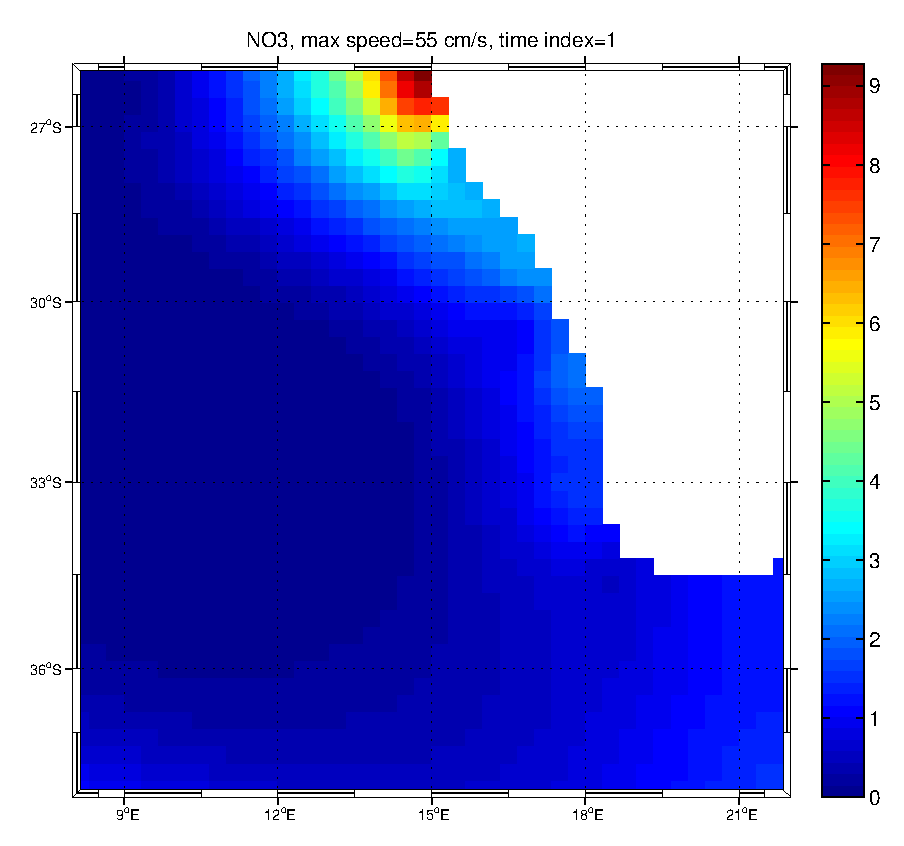
\includegraphics[width=0.5\textwidth]{NO3_surf_t1.eps}}%
\hfill
\subfigure[vertical sections along open boundaries]{
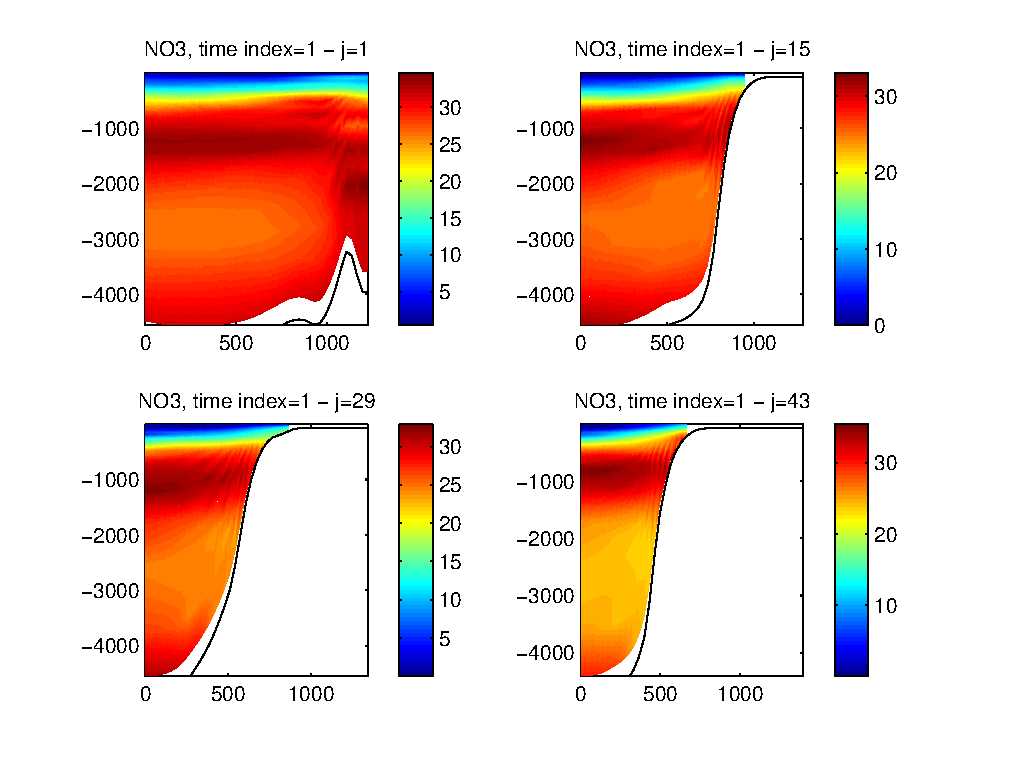
\includegraphics[width=0.5\textwidth]{NO3_profil_t1.eps}}
\caption{Result of make\_clim\_pisces for the Benguela example : NO3 forcing
  fields [mMol N m-3].}
\label{fig:makeclimpiscesNO3}
\end{figure}


\begin{figure}[!htbp]
\subfigure[Surface map]{
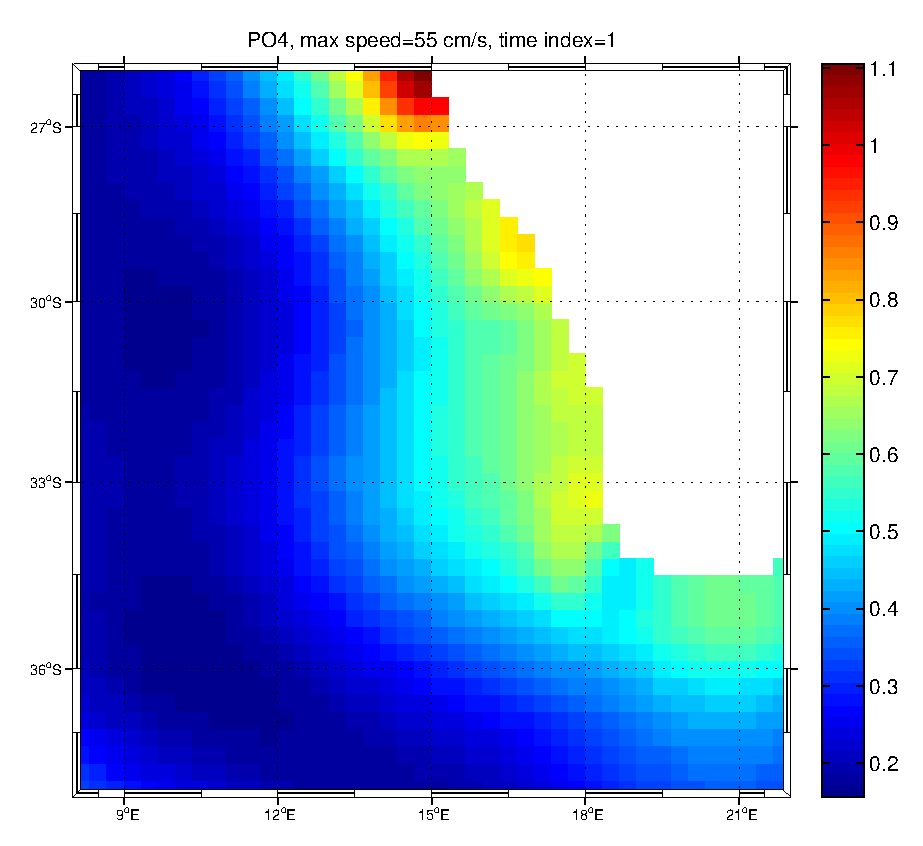
\includegraphics[width=0.5\textwidth]{PO4_surf_t1.eps}}%
\hfill
\subfigure[vertical sections along open boundaries]{
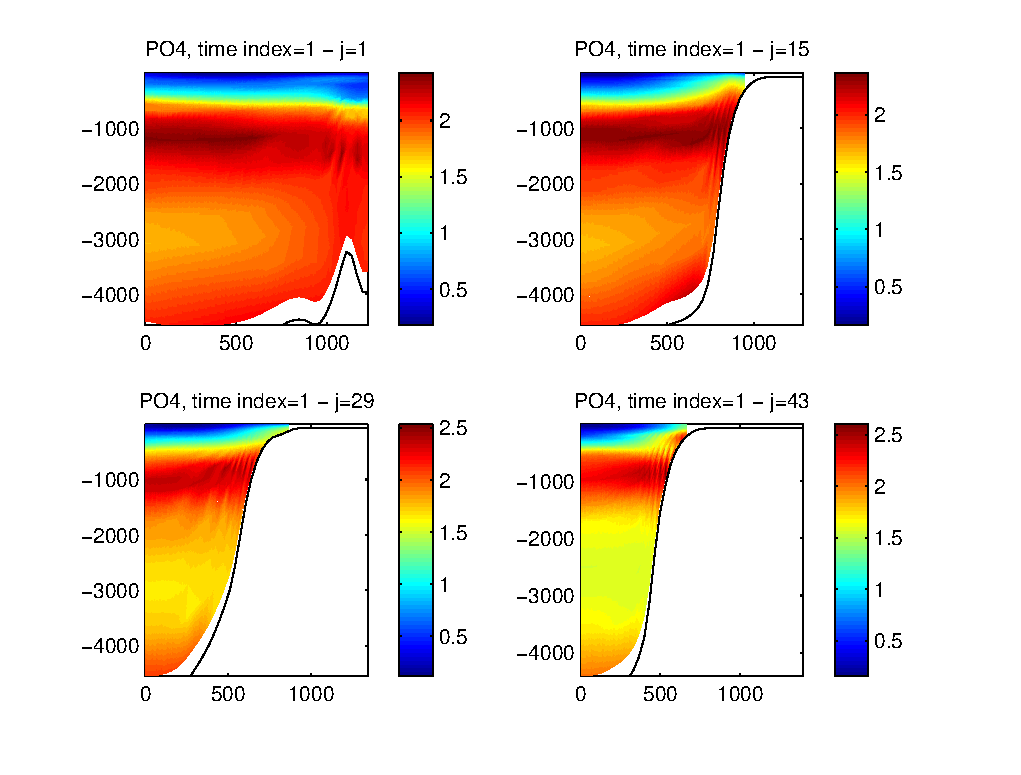
\includegraphics[width=0.5\textwidth]{PO4_profil_t1.eps}}
\caption{Result of make\_clim\_pisces for the Benguela example : PO4 forcing fields
  [mMol P m-3].}
\label{fig:makeclimpiscesNO4}
\end{figure}

\noindent Finally, to compute the Iron dust deposition forcing file roms\_frcbio.nc file, in a matlab session,  run make\_dust.m :\\
$>>$\\
$>>$ make\_dust\\
\begin{figure}[!htbp]
\centering
\subfigure{
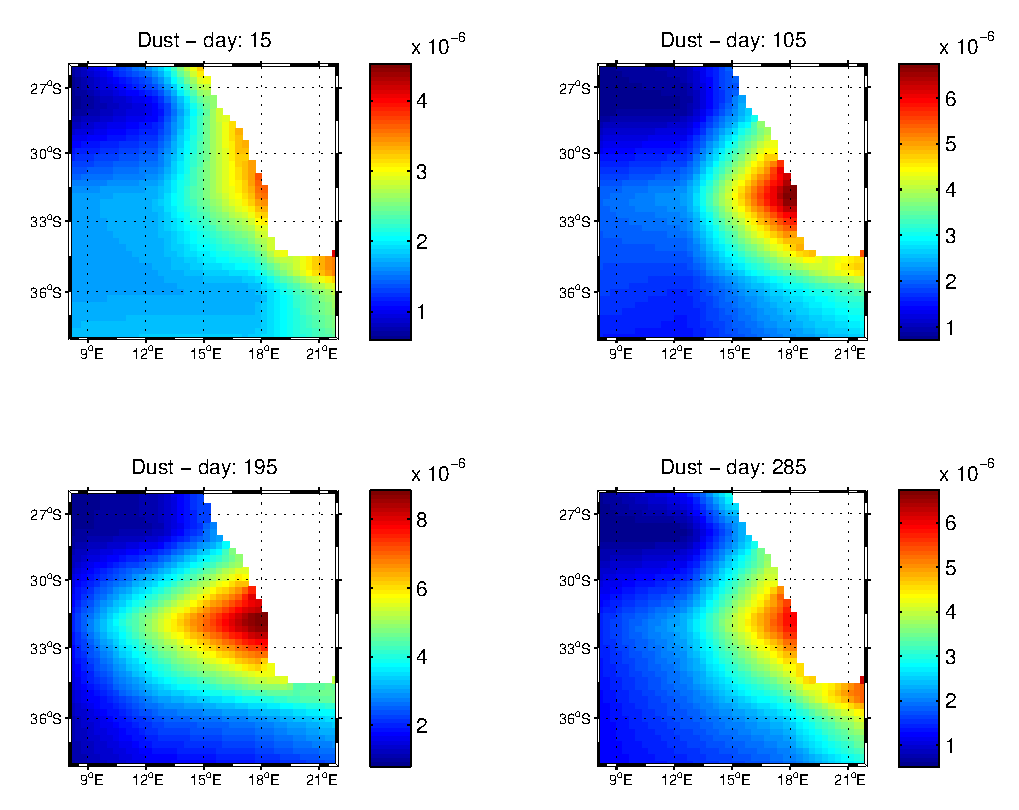
\includegraphics[width=1\textwidth]{dustdepo_surface.eps}}%
\hfill
\caption{Result of make\_clim\_pisces for the Benguela example : Iron dust deposition
  forcing fields [nmol Fe m-3].}
\label{fig:makeclimpiscesNO4}
\end{figure}

If the makepisces =1 in romstools\_param.m,   \textbf{make\_clim.m} will process directly  \textbf{make\_clim\_pisces.m}, \textbf{make\_dust.}m and eventually \textbf{make\_ini\_pisces.m}.
It is exactly the same procedure for the roms\_bry.nc files. \\

The cpp keys related to this biogeochemical model are :
\begin{itemize}
\item PISCES : Select the PISCES biogeochemical model
\item DIAGNOSTICS\_BIO : Define if writing out fluxes between the biological
components. \\
\end{itemize}
